\section{Flight Day}

The balloon launch base in Timmins, Ontario is located at 48.47\si{\degree}N 81.33\si{\degree}W and ALI arrived at the base located at the Victor M. Power Airport on August 25, 2014 with a launch window from September 8 to 14, 2014. In between the arrival and launch ALI was integrated onto the CNES CARMEN gondola with four other instruments, including one other from the University of Saskatchewan. When ALI was integrated with CARMEN's systems, including communications and power and ALI was orientated so it would be 90\si{\degree} from the direction of the sun in regard to the gondolas pointing system with an overall southern field of view during the mission. CARMEN is a gondola with pointing capabilities and is piloted from the ground station in Timmins during the flight. The pointing precision is then fine tuned to a pointing of better than 1\si{\degree} with the use of an onboard star tracker.

The flight of CARMEN was delayed due to poor weather conditions during the launch window. On September 20, 2014 at 05:35 UTC (01:35 local time) ALI was launched as the Nimbus 7 mission onboard the CNES CARMEN gondola from the CSA Timmins balloon launch facility. During the launch, the sky was clear with light winds allowing for an safe and uneventful launch. The ascent of CARMEN occurred in darkness and reached its flight altitude of 36.5~km at 8:17 UTC. First light was observed by ALI at 9:39 UTC and recorded measurements until 14:42 UTC when the primary aerosol mission was completed. ALI was powered off at 17:15 UTC during this time ALI recorded measurements for secondary goals, including an azimuth scan. A visualization of the flight path with all major landmarks noted can be found on \autoref{fig:5.1:nimbus7FlightPath}. Temperature profiles for the ambient atmosphere and instrument can be seen in \autoref{fig:5.1:nimbus7Temps}. The black curve is the ambient atmospheric temperature surrounding the gondola during the flight from the ECMWF \citep{Molteni1996}. The blue, green, and red are from temperature sensors onboard ALI located on the baffle, camera, and RF driver respectively. The baffle temperature sensor was attached just on the inside of the ALI right by the entrance aperture for the system and monitors the temperature at the front of the system. The camera sensor is attached to the back of the CCD camera and the RF driver sensors measures the temperature of the RF driver. ALI was thermally insulated with styrofoam to keep the system warm, while at the same time direct heating from the sun was a concern and the system was covered in a reflecting material to reduce solar heating.

During the mission, ALI ran in two primary operational modes, a dark mode and a aerosol imaging mode. The first mode, the dark mode was primarily used during assent and intermittently between aerosol modes. During this mode the filtering of the AOTF is disabled, meaning with no RF signal being applied to the crystal, and as such the wavelength has no dependance on the images. Eight exposures are taken at with 0.05, 0.1, 0.5, 1, 2, 3, 5, 10 second exposure times with the camera shutter operating. The second operational mode was the aerosol mode and it records 13 measurements which each consisted of a pairs of images. A pair of images, one with the AOTF enabled and one disabled, were gathered for every 25~nm between 650 to 950~nm each measurement set took approximately 25~s to acquire. The exposure times were determined by making ground based measurements of all of the wavelengths in the aerosol mode at a variety of exposure times. This data was used to determine the value at which the well of the CCD would be three quarters full on the ground. Then using the known geometry from the ground and assumed geometry from the balloon in combination with the SASKTRAN model, which will be discussed in \autoref{TODO:??}, simulated radiance profiles for both geometries were determined. The determined ground based exposure times were scaled to balloon exposure times by the ratio of the balloon based modeled radiances over the ground based modeled radiances. % A unique feature of the AOTF is that the diffraction can be disabled to take an image with the filter disabled. These so called `dark images' allows capture of the stray light which are use in processing to accurately and easily remove stray light from the signal, as such a `dark image' was also gathered in between each filter acquisition for assist in the calibration of the measurements.


\begin{figure}
    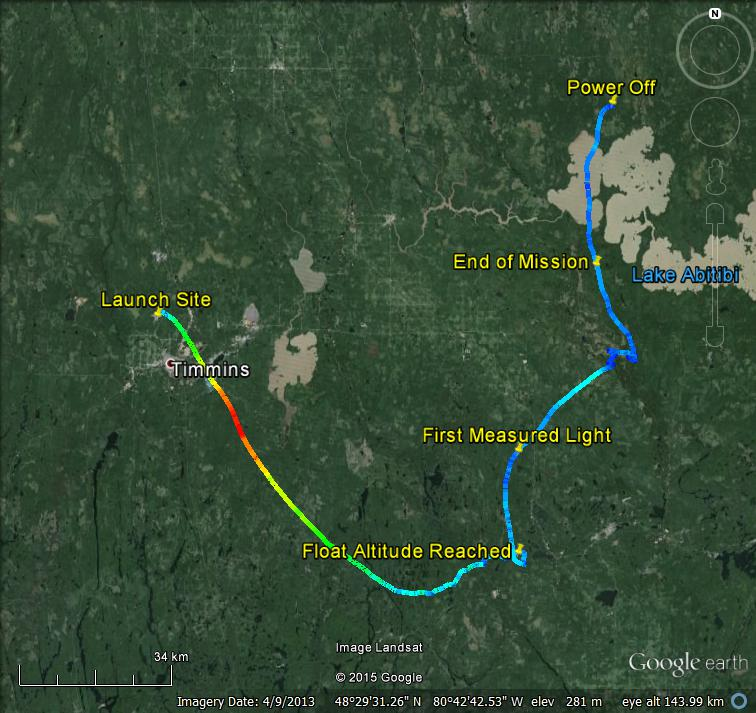
\includegraphics[width=1.0\textwidth]{./Images/5-1-AliGpsDataGoogleMaps.jpg}
    \caption[Flight Path of the Nimbus 7 Mission]{The GPS data from ALI during the Nimbus 7 mission generated via Google Earth. The colour of the line represents the absolute speed of the gondola during the mission. Important landmarks noted on the image. The end of mission represent the end of the primary aerosol mission. No GPS data was collected from ALI after the power down.}
    \label{fig:5.1:nimbus7FlightPath}
\end{figure}

\begin{figure}
    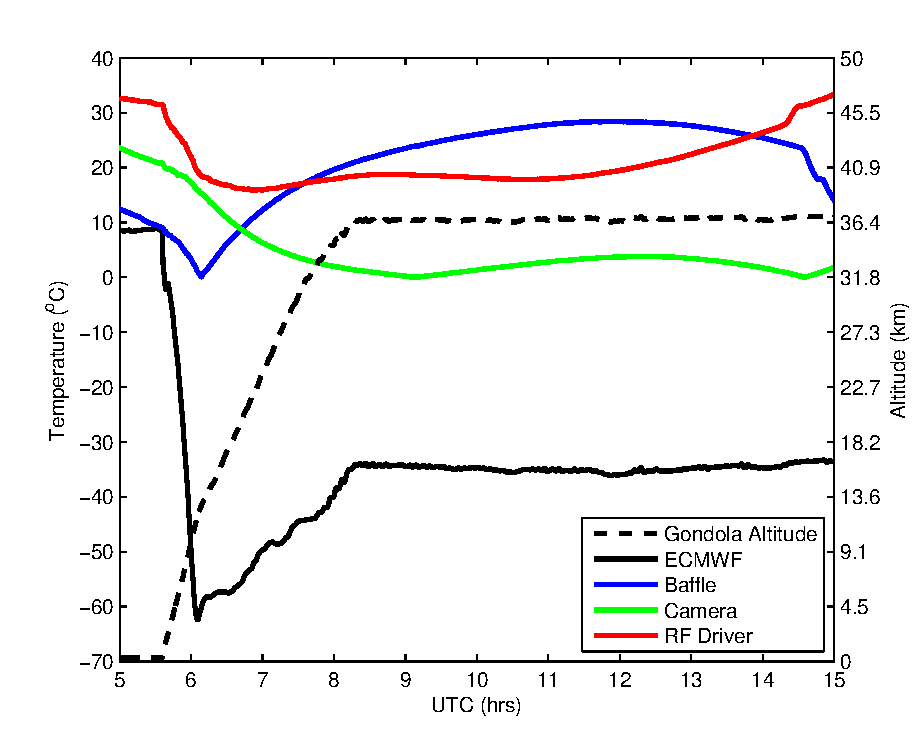
\includegraphics[width=1.0\textwidth]{./Images/5-1-FlightTemperatures.pdf}
    \caption[Flight Temperatures and Altitude Profiles from Nimbus 7]{Temperature and altitude profiles from the NIMBUS 7 flight.}
    \label{fig:5.1:nimbus7Temps}
\end{figure} 